\section{Risposta a segnali sinusoidali di frequenza fissa.}
\subsection{a}
In questa sezione si è studiato il fattore di amplificazione a frequenza costante.
Per prima cosa si è verificato che effettivamente il filtro inverta di $\pi$ la fase del segnale. Questo fenomeno è mostrato in \ref{f:Inv}.\\
\begin{figure}
\centering
	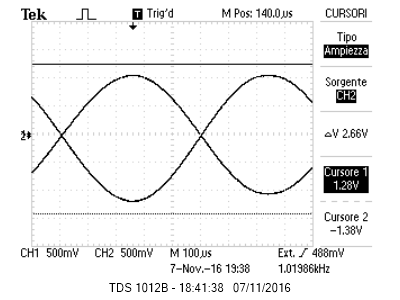
\includegraphics[scale=1]{inversion.png}
	\caption{Il canale 2 è chiaramente invertito rispetto al canale 1.\label{f:Inv}}
\end{figure}
Si sono prese le tensioni(picco picco) $V_{out}$ in variando $V_{in}$. Entrambe le misure di tensione sono state prese con l'oscilloscopio. L'errore di calibrazione è stato trascurato poiché molto minore del rumore. La stima del suddetto rumore è stata fatta misurando la semidifferenza tra il valore massimo ed il valore minimo della banda di rumore.%.\marginpar{spiego quì della 0.67?}\\

Si è dunque provveduto a fittare i parametri $\alpha, \beta$ dell'equazione $V_{out}=\alpha V_{in} + \beta$. Chiaramente questa espressione ha una regione di validità limitata (dal semplice fatto che forti oscillazioni della corrente di base possono portare il transistor in saturazione o in interdizione), dunque si è dovuto stabilire un tetto massimo alle tensioni da considerare nel fit. Inizialmente questo limite è stato posto arbitrariamente a $\SI{1.5}{\V}$. Dopo un primo fit si è poi variato questo tetto massimo e si è controllato che, per ogni tetto massimo, il fit desse risultati compatibili entro l'errore e valori del $\chi^2$ significativi.\\
Per il primo fit si è ottenuto:\\
$\alpha=9.53 \pm 0.08$\\
$\beta=\SI{0.04 \pm 0.03}{\V}$\\
$\chi^2= 4.9$ ($7$ DoF, $p_{\chi^2>4.9} = 0.67)$\\

Si vede come $\beta$ sia quasi compatibile con 0, mentre $\alpha$ sia vicino al valore di riferimento, $10$, dato nel testo. La misura precisa delle resistenze relativamente $R_C=\SI{9.98\pm 0.09}{\kohm}$ ed $R_E=\SI{989 \pm 9}{\ohm}$, fornisce $\alpha=10.08 \pm 0.14$; in figura \ref{f:VinVout} i dati e il fit.

\begin{figure}
\centering
	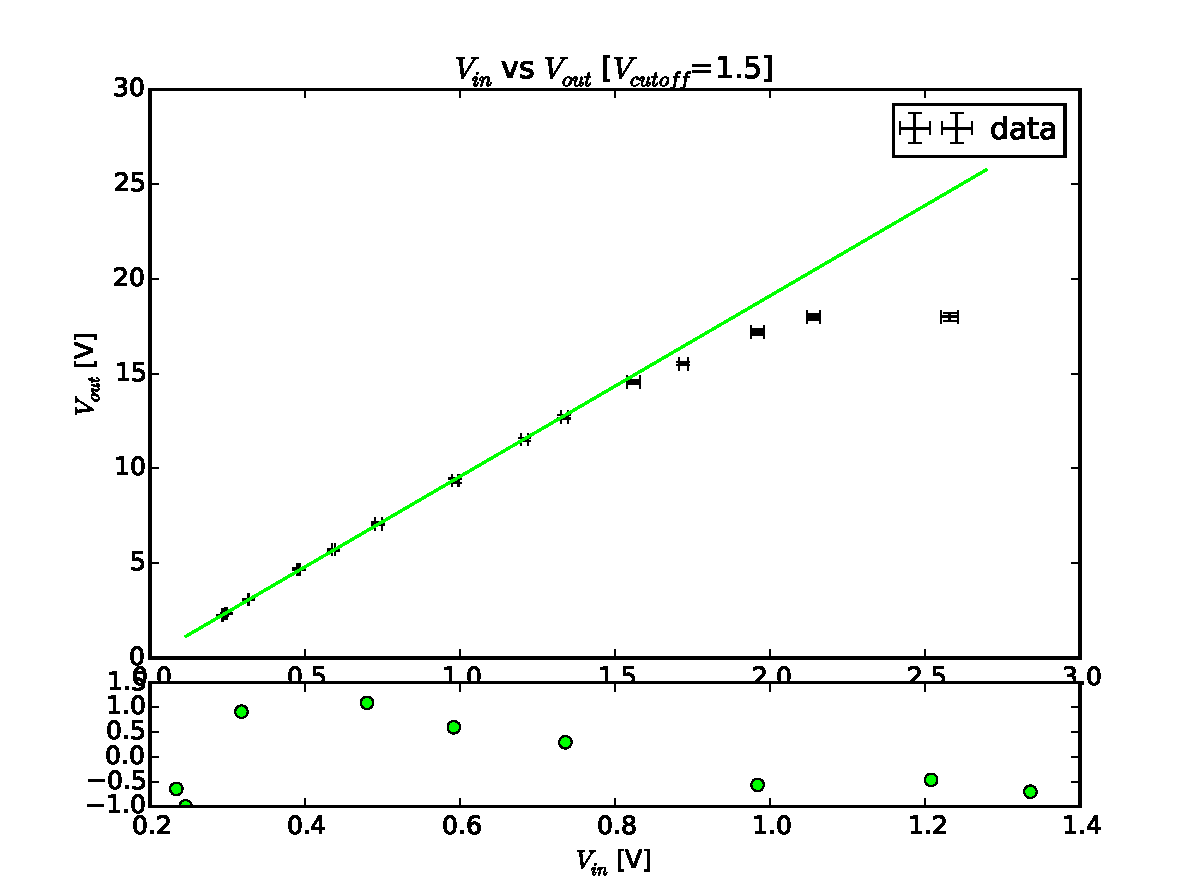
\includegraphics[scale=0.8]{VinVout.pdf}
	\caption{Andamento lineare, fittato con un cutoff di $\SI{1.5}{\V}$.\label{f:VinVout}}
\end{figure}

Si è dunque provato a fittare valori diversi di $V_{cutoff}$ (selezionando dunque i punti sperimentali massimi presi) e si è visto:\\

\begin{tabular}{l l l l l l l l}
$V_{cutoff}$ 	&	$\alpha$	&	$\sigma_\alpha$	&	$\beta$ & $\sigma_\beta$ & $corr$ & $\chi^2$ & p\\
\hline
1.6 & 9.48 & 0.7 & 0.06 & 0.1& -0.83 & 17.71 & 0.02\\
1.3 & 9.56 & 0.1 & 0.03 & 0.03 & -0.87 & 4.4   & 0.62\\
1.1 & 9.61 & 0.3 & 0.02 & 0.05& -0.91 & 3.5   & 0.622\\
0.9 & 9.67 & 0.14& 0.00 & 0.05& -0.93 & 2.1	& 0.724\\
\end{tabular}
\\
%1.6 ChiSquare = 17.719348475581825 (8 DoF, p = 0.02343185643860659)[ 9.48435779  0.05830901] [[ 0.00541004 -0.00201242] [-0.00201242  0.00109663]] cor=1.4649593148410518
% 1.3 ChiSquare = 4.380144835013295 (6 DoF, p = 0.6253769516198249)[ 9.56460543  0.03315335] [[ 0.00991501 -0.00341248] [-0.00341248  0.00153505]] cor=1.3070022498913363
%1.1	ChiSquare = 3.5054382142416274 (5 DoF, p = 0.6225649168737695)[ 9.61808402  0.01700887] [[ 0.01681629 -0.00550071] [-0.00550071  0.00216913]] cor=1.2055296121994161
%ChiSquare = 2.062422135768341 (4 DoF, p = 0.7242788074577765)[  9.69923847e+00  -6.81361111e-03] [[ 0.02440091 -0.00773502] [-0.00773502  0.00283078]] cor=1.154488654253337

Questi dati ci portano a concludere che entro $1.5 V$ la relazione lineare è ben verificata, oltre si verifica qualcosa di atteso, già presente a $1.6 V$. Per analizzare questo fenomeno bisogna ricordare quale è il punto di funzionamento del transistor. Per i componenti presi in esame, infatti, le resistenze prese portano il diodo a lavorare con un $V_{ce}=\SI{8.02\pm 0.05}{V}$ e $I_e=\SI{1.112\pm 0.01}{\mA}$. Questo ci dice subito che mandando un segnale alternante, nella semi-onda positiva del segnale di ingresso, non si potrà ottenere un elongazione, nel segnale amplificato, maggiore di circa $8V$ poiché, prima di tale tensione, si raggiunge la saturazione del transistor.  Similmente non si potrà ottenere una elongazione superiore a $-12V$ nella semi-onda negativa, in quanto si raggiunge la completa interdizione. In generale ci si aspetta dunque di ottenere una ampiezza picco-picco massima del segnale amplificato di $20V$ (con un significativo clipping della semi-onda negativa in uscita). Ci si aspetta inoltre di vedere comparire il clipping prima nella semi-onda negativa, poi in quella positiva. In effetti dalle immagini acquisite \ref{f:Cli}:

\begin{figure}[h]
\centering
	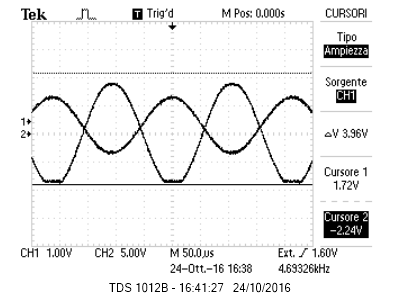
\includegraphics[scale=1]{clipping_1.png}
	\caption{Si nota il clipping nella semionda negativa, non ancora quello nella semionda positiva.\label{f:Cli}}
\end{figure}

\begin{figure}[h]
\centering
	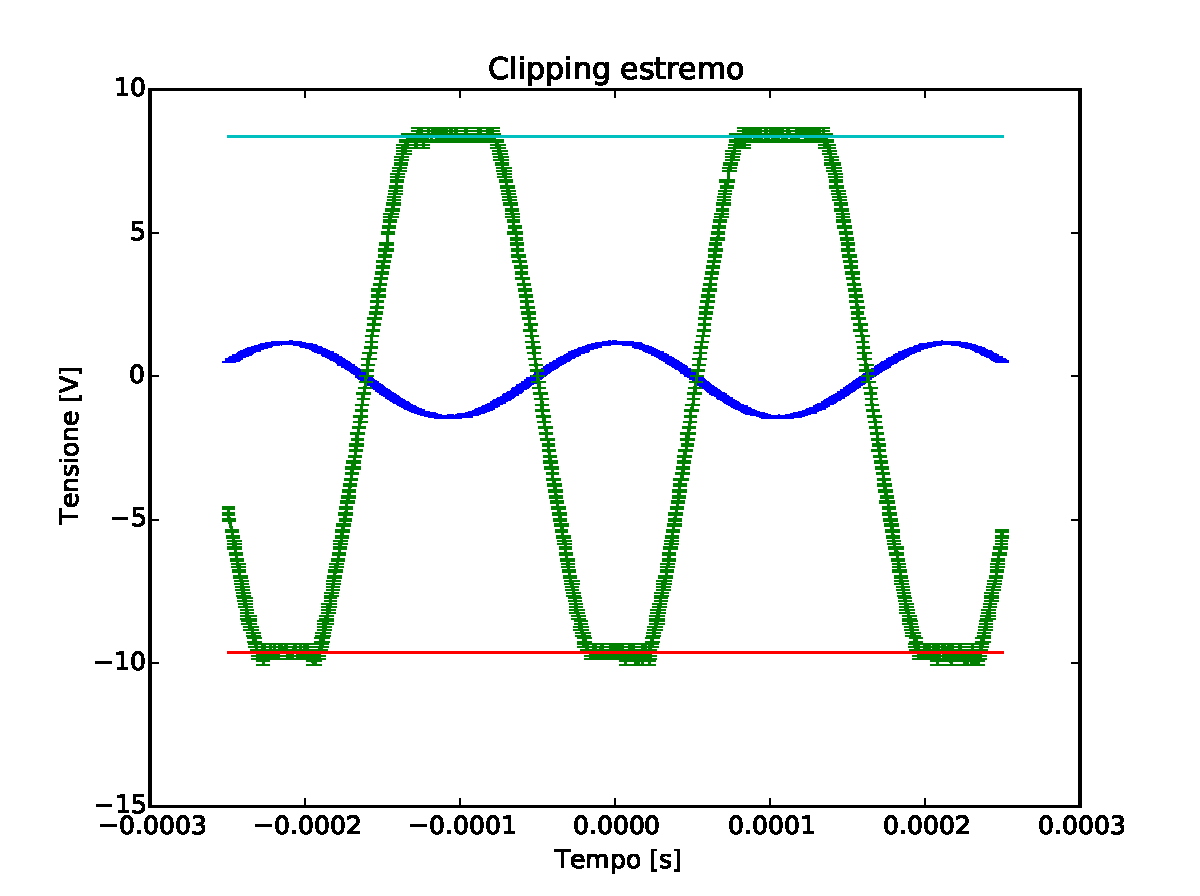
\includegraphics[scale=0.8]{clipping.pdf}
	\caption{Clipping sia nella semionda positiva che in quella negativa.\label{f:Cli2}}
\end{figure}

Si è dunque provato a trovare il valore di tensione in uscita per cui si ottiene clipping totale in alto che in basso. Per fare questa misura si sono usati i dati in figura \ref{f:Cli2}(Acquisiti con l'oscilloscopio e importati dal computer per mezzo del programma OpenChoice).\\
I risultati ottenuti sono:\\
$V_{min}=\SI{-9.64\pm 0.1}{V}$\\
$V_{max}=\SI{ 8.37\pm 0.1}{V}$\\
Compresi di errori di calibrazione dell'oscilloscopio.

Si nota che la tensione $V_{min}$ è minore (in modulo) di quella aspettata, mentre la $V_{max}$ è maggiore. Quest'ultimo comportamento è compatibile con un entrata del transistor in saturazione prima che $V_{ce}=0$.

\subsection{b}
In questa sezione si cerca di valutare la resistenza di ingresso del circuito. La resistenza attesa, trascurando i condensatori, è:\\
$R_{in}=(h_{ie}+R_E \cdot h_{fe}) \paral R_1 \paral R_2$\\
Trascurando anche $h_{ie}$ (molto minore di $R_E\cdot180$) ed usando il valore stimato di 178 per $h_{fe}$ (pari all'$h_{FE}$ misurato nella scorsa esperienza), si ottiene:\\
$R_{in} =\SI{ 14.65(15)}{\kohm}$\\
Sperimentalmente questa grandezza è stata misurata valutando il rapporto tra la tensione in uscita (ritenuta proporzionale a quella in ingresso alle ampiezze a cui lavoravamo) del circuito normale e la tensione in uscita osservata mettendo in serie al generatore una resistenza $R_x=\SI{15.33\pm 0.01}{\kohm}$. Si è ottenuto un segnale $V_{out}=\SI{2.26 \pm 0.1}{\V}$ contro un segnale originario di  $V_{out}=\SI{4.64 \pm 0.12}{\V}$. La resistenza di ingresso è dunque:\\
$R_{in}=\frac{R_x}{V_1/V_2-1}=\SI{14.5\pm 0.3}{\kohm}$, compatibile con quanto previsto.

La nostra stima è stata effettuata senza tener conto della reattanza del condensatore: la componente reattiva, infatti, in serie a tutta l'impedenza $R_{in}$ è $Z_c= \inv{j \omega C} = \SI{-0.90(5)j}{\kohm}$.

Il modulo dell'impedenza in ingresso, tenendo conto di $Z_c$, è \SI{14.67(15)}{\kohm}; la variazione essenzialmente nascosta dall'errore autorizza l'aver trascurato il condensatore nei calcoli precedenti.

\subsection{c}
In questa sezione ci si prefigge il compito di misurare la resistenza di uscita del circuito.\\
Si è misurata mettendo in parallelo una resistenza da $R_x=\SI{9.88\pm 0.01}{\kohm}$ e misurando $V_1$ e $V_2$ le tensioni di uscita prima e dopo l'inserimento.\\
Si sono ottenute le seguenti misure:\\
$V_1=\SI{4.64\pm 0.12 }{\V}$	$V_2=\SI{2.32\pm 0.06}{\V}$\\
Che portano a una resistenza di:\\
$R_{out}=R_x(V_1/V_2-1) = \SI{9.9 \pm 0.7}{\kohm}$, pienamente compatibile con il valore atteso $R_C$ (\SI{9.98 (9)}{\kohm}). L'impedenza reattiva del condensatore in uscita è di nuovo trascurabile.






